% !TeX root = ../main.tex

\chapter{绪论}

\section{研究背景}

作为计算机图形学的子领域之一,渲染是将用不同表达表示的几何、材质、光照、相机等信息综合,然后最终生成二维图像的过程。根据单幅图像的渲染时间来分类,计算机图形学领域通常将渲染技术分为实时渲染和离线渲染两个大类。对于实时渲染来说,实时性是需要保证的重要性能指标,而这一般意味着绘制帧率需要达到每秒 30 幅画面或更高。例如,图 \ref{fig:blender_online_vs_offline} 给出了 Blender 软件中的离线渲染器 Cycles 和实时渲染器 Eevee 渲染场景中玻璃材质的茶壶时的画面表现的对比。Cycles 使用路径追踪(Path tracing)算法进行渲染,虽然更加真实,但是渲染该场景的时间远远高于主要基于光栅化渲染流水线的 Eevee。

\begin{figure}[htbp]
    \centering
    \begin{minipage}[b]{\textwidth}
        \begin{subfigure}[b]{0.48\textwidth}
            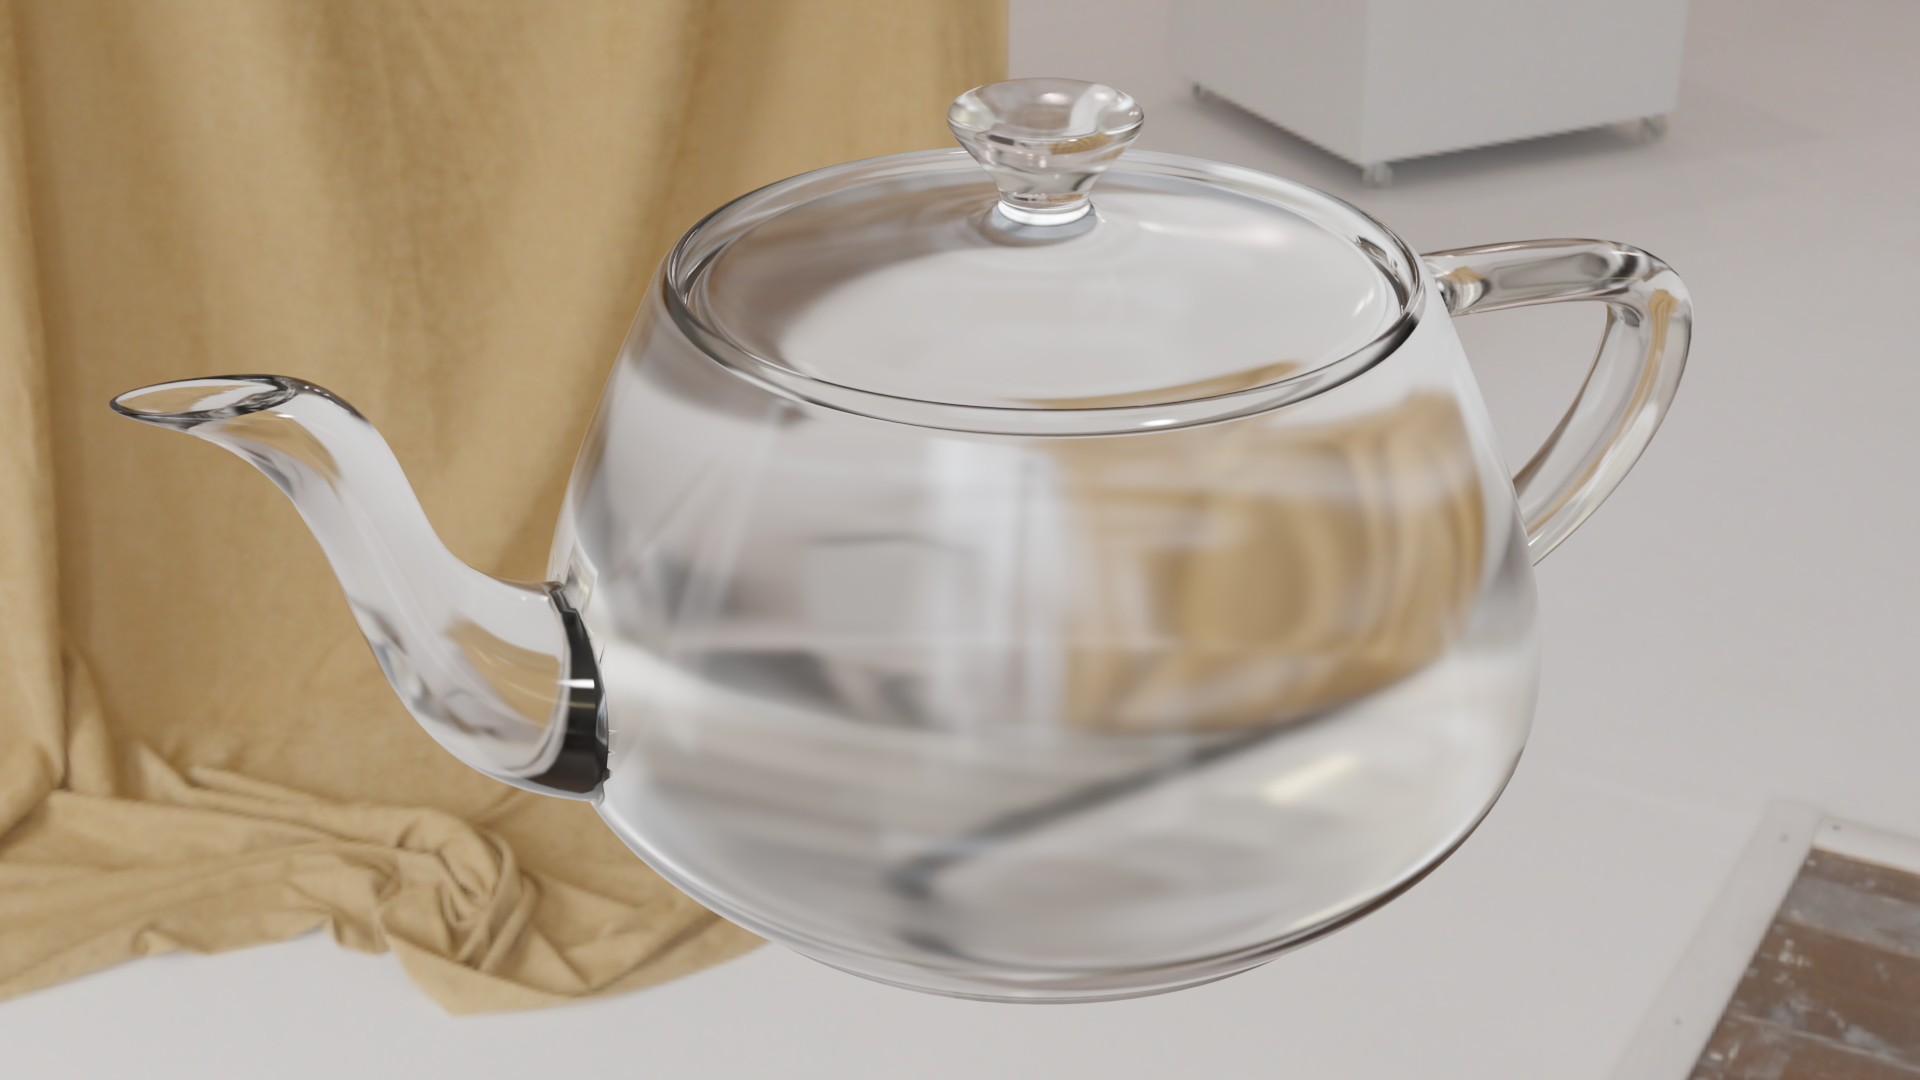
\includegraphics[width=\textwidth]{figures/BlenderTeapot-15-50s-Offline.png}
            \caption{Cycles 渲染示例 (用时 15min50s)}
            \label{fig:sub_cycles}
        \end{subfigure}
        \hfill % Adds horizontal space between the subfigures
        \begin{subfigure}[b]{0.48\textwidth}
            \includegraphics[width=\textwidth]{figures/BlenderTeapot-220ms-Online.png}
            \caption{Eevee 渲染示例 (用时 220ms)}
            \label{fig:sub_eevee}
        \end{subfigure}
    \end{minipage}
    
    %\vspace{1em} % Adds vertical space between the rows of subfigures
    
    \caption{Blender 软件中离线渲染器 Cycles 和实时渲染器 Eevee 效果和时间对比}
    \label{fig:blender_online_vs_offline}
\end{figure}


利用专用的 GPU 和光栅化渲染流水线来进行实时渲染是目前的主流方案。这种方案将实时渲染过程抽象为以顶点输入、顶点着色、光栅化、片段着色和深度模板测试为主要阶段的绘制流水线过程。为了方便对不同厂商生产的 GPU 进行编程,设备和操作系统厂商间约定了比较稳定的图形 API,例如现在由 Khronos Group 负责的 OpenGL\cite{OpenGLSpec},OpenGL ES\cite{OpenGLESSpec},Vulkan\cite{VulkanSpec},由 Microsoft 公司负责的 Direct3D\cite{Direct3DSpec} 和由 Apple 负责的 Metal\cite{MetalSpec} 等。


早期的图形流水线设计多以固定流水线功能为主,图形程序员只能够操作流水线功能的开启和关闭,并不能自己编写程序对顶点和片段颜色等进行流水线预设功能之外的操作。随着图形硬件的功能演进,OpenGL 和 Direct3D 均加入了通过图形程序员编写的专用程序片段来替换部分固定流水线实现的功能。这样的专用程序片段被称为着色器程序(Shader Program)。

对于现代图形 API 来说,着色器程序本身以 HLSL,GLSL 等高层次描述语言写就,并在程序运行时呈递给设备厂商或操作系统厂商提供的驱动程序中的编译器进行运行时编译。多种多样的着色器程序极大的丰富了光栅化图形流水线可以实现的图形和图像效果,成为了现在游戏、VR 等交互式互动娱乐应用程序编写时的重要组成部分。

为了适应实时渲染在各种类型终端上的广泛需求, GPU 市场十分丰富。对于桌面端,就有 Intel, AMD, NVIDIA, Apple 等公司提供 GPU 解决方案;而如 Qualcomm,Broadcom,Imagination,华为海思等公司则提供移动端的 GPU 和 IP 解决方案。

\begin{figure}[htbp]
    \centering
    \begin{minipage}[b]{\textwidth}
        \begin{subfigure}[b]{0.34\textwidth}
            \includegraphics[width=\textwidth]{figures/10700-cpu-front.jpg}
            \caption{搭载 UHD 核显的 Intel CPU}
            \label{fig:sub_10700}
        \end{subfigure}
        % \hfill % Adds horizontal space between the subfigures
        \begin{subfigure}[b]{0.32\textwidth}
            \includegraphics[width=\textwidth]{figures/PURE-AMD-Radeon™-RX-7900-GRE-1-scaled.jpg}
            \caption{AMD Radeon 独立显示卡}
            \label{fig:sub_7900gre}
        \end{subfigure}
        % \hfill
        \begin{subfigure}[b]{0.33\textwidth}
            \includegraphics[width=\textwidth]{figures/Kirin-9000S.png}
            \caption{搭载马良 GPU 的麒麟 SoC}
            \label{fig:sub_kirin9000s}
        \end{subfigure}
    \end{minipage}
    
    %\vspace{1em} % Adds vertical space between the rows of subfigures

    % TODO: add reference
    \caption{不同形态终端设备中搭载的 GPU 产品\cite{sapphire2024radeon, tpu2020intelcorei710700, bilibili2023huaweimate60pro}}
    \label{fig:gpu_gallery}
\end{figure}

{\amend 上述} GPU 家族,包括其各自每代的处理器设计,通常拥有不同的指令集架构(Instruction Set Architecture,ISA),微架构等,而仅仅在图形 API 的层次上做到对使用者一致。例如,桌面端的 GPU 普遍支持 Direct3D,Vulkan,OpenGL 等图形 API,移动端的 GPU 则普遍支持 OpenGL ES, Vulkan 等图形 API。对于应用开发者来说,设备厂商通过图形 API 层来努力隔离设备之间的异质性。例如,图 \ref{fig:drivers_overview} 给出了 Linux 平台下图形应用程序通过 Vulkan API 来使用 Intel 和 AMD 独立显卡时所分别经过的软件栈。可以看到,此处的两个不同厂商拥有不同的用户态驱动程序和内核态驱动程序,但可以统一经由 Vulkan 装载器来向图形应用程序暴露 Vulkan 接口,以简化程序开发人员的程序编写工作。

\begin{figure}
    \centering
    \includegraphics[page=2, width=0.8\linewidth]{figures/pictures.pdf}
    \caption{使用 Vulkan 的图形应用程序在 Linux 平台下调用 Intel 和 AMD 显卡示例}
    \label{fig:drivers_overview}
\end{figure}

然而,这种隔离并不是充分的。不同的架构和单元配置会影响 GPU 执行用户负载时的性能,而这种性能上的区别会对最终用户的体验产生或多或少的影响。在所有图形程序的性能影响因素中,着色器程序因其可编程性,会对性能产生较大的影响。因此,本文围绕着光栅化绘制流水线中的着色器程序,研究其性能的预测问题。

\section{{\amend 挑战与研究内容}}

\label{sec:challenge}

针对于 GPU 上应用的性能预测和优化问题,业界已经开发出多种工具和方法。以 Radeon Graphics Profiler\cite{AMDRGP} 和 NSight Graphics\cite{NSightGraphics} 为例,它们会通过一次或多次专门的绘制流水线剖析过程,利用 GPU 内部的性能计数器给出着色器的优化建议。此外,诸如 Emerald \cite{10.1145/3307650.3322221} 和 GPGPU-Sim \cite{4919648} 这样的体系结构模拟器,则通过对 GPU 架构的模拟和较精确的建模来预测着色器的性能。然而,上述方法和工具的局限性在于,其依赖于特定的厂商或 GPU 架构,且需要在每一种 GPU 上进行单独测试或专门的模拟运行。这样一来,在高度分散的 GPU 市场中,这种特性要求开发者对每一种平台都进行单独的建模或性能分析,增加了额外的测试和调优负担。

在着色器优化和简化问题过程中,学术界曾有相关研究对待优化的着色器性能进行建模\cite{10.1145/2816795.2818104, 10.1111/cgf.13482, 10.1145/3528233.3530722}。然而,这些工作主要采用较简单的性能估算方法,比如认为着色器的运行时间和着色器中进行的标量运算以及纹理访问操作次数成正比。然而,着色器指令的执行时间受到多种因素的影响。这些影响因素包括编译器优化和 GPU 架构特征,如缓存系统设计和运算单元的数量等。因此,这些未能充分考虑这些因素的模型,往往不能准确预测性能表现。

{\amend 基于上面的观察,本文认为利用数据驱动的方法可以较为有效的解决上面存在的两类挑战。故而,本文提出了下面两个工作:}

{\added 其一,本文构建了面向性能预测的着色器性能数据集,通过设计的较为严谨的收集和性能测量过程,获得了 5 个平台共 54667 个性能样本的,丰富的片元着色器性能数据集。同时,基于该数据集,本文筛选并构建了着色器性能挑战样本集,其包含有在不同平台性能差异较为明显的样本。同时,为了了解着色器的功能分布特征,本文探究了使用基座语言模型来进行着色器类别标注的工作。}

{\amend 其二,本文提出了一种数据驱动的、}针对不同 GPU 平台上绘制流水线中着色器的性能进行建模和预测的方法。在数据驱动的基础上,{\amend 利用本文构造的指令计数追踪和 Transformer 的指令计数嵌入环节,该方法可以平台独立的应用到各种不同 GPU 平台。}同时,通过在着色器性能样本上进行训练,GPU 架构特征和程序负载特征等和程序性能相关的因素也被纳入考虑,从而较现有方法提高了预测效果。

\section{{\amend 章节安排}}

本文的章节安排大致如下:

第一章主要介绍本研究的研究背景、研究意义,挑战和研究的大致内容。

第二章主要介绍本研究相关的背景知识和相关工作。本研究主要和着色器程序优化,程序语言理解和程序性能建模三个方面相关。

{\added 第三章主要介绍本研究构建的,面向性能预测的着色器性能数据集。该章首先介绍了着色器程序数据集的收集和理解工作中面临的诸多挑战,并介绍了本章工作应对这些挑战的方面。之后,该章详细介绍了着色器收集和性能测量环节的具体实现、挑战样本集的构造,以及利用基座语言模型进行着色器类别标注的相关探索。最后,该章仔细分析了着色器数据集的分布特征,其受到其它因素所导致的性能波动的程度,着色器过滤和挑战样本的情况,以及基座语言模型对于类别标注问题的实践结果。}

第四章主要介绍本研究提出的,数据驱动的着色器程序性能预测方法。该章首先介绍了着色器程序性能预测面临的问题和该方法的设计思路,随后分别介绍了该方法较核心的两部分的设计,分别为基本块粒度的 SPIR-V 指令追踪的程序编排和实现,以及该方法构造的{\amend 基于 Transformer 的着色器程序性能预测模型}。最后,本章给出了上面提到的部分的实验和分析{\amend,其中包括基线、消融实验和若干对比实验。}

第五章给出了本研究的工作总结和展望。